\section{Properties}\label{properties}

GObject system provides properties. Properties are values kept by
instances, which is a descendant of GObject, and they are open to other
instances. They can be accessed with their names.

For example, GtkWindow has ``title'', ``default-width'',
``default-height'' and other properties. The string ``title'' is the
name of the property. The name of a property is a string that begins
with a letter followed by letters, digits, dash (`-') or underscore
('\_'). Dash and underscore is used as separators but they cannot be
mixed. Using dash is more efficient than underscore. For example,
``value'', ``double'' and ``double-value'' are correct property names.
``\_value'' or ``-value'' are incorrect.

Properties have various types of values. The type of ``title'' property
is string. The type of ``default-width'' and ``default-height'' is
integer.

Properties are set and got with functions defined in GObject.

\begin{itemize}
\tightlist
\item
  Properties can be set with several GObject functions.
  \passthrough{\lstinline!g\_object\_new!} and
  \passthrough{\lstinline!g\_object\_set!} are often used.
\item
  Properties can be get with several GObject functions.
  \passthrough{\lstinline!g\_object\_get!} is often used.
\end{itemize}

The functions above belongs to GObject, but they can be used for any
descendant object of GObject. The following is an example of GtkWindow,
which is a descendant object of GObject.

An instance is created and its properties are set with
\passthrough{\lstinline!g\_object\_new!}.

\begin{lstlisting}[language=C]
GtkWindow *win;
win = g_object_new (GTK_TYPE_WINDOW, "title", "Hello", "default-width", 800, "default-height", 600, NULL);
\end{lstlisting}

The example above creates an instance of GtkWindow and sets the
properties.

\begin{itemize}
\tightlist
\item
  The ``title'' property is set to ``Hello''.
\item
  The ``default-width'' property is set to 800.
\item
  The ``default-height'' property is set to 600.
\end{itemize}

The last parameter of \passthrough{\lstinline!g\_object\_new!} is
\passthrough{\lstinline!NULL!} which is the end of the list of
properties.

If you have already created a GtkWindow instance and you want to set its
title, you can use \passthrough{\lstinline!g\_object\_set!}.

\begin{lstlisting}[language=C]
GtkWindow *win;
win = g_object_new (GTK_TYPE_WINDOW, NULL);
g_object_set (win, "title", "Good bye", NULL);
\end{lstlisting}

You can get the value of a property with
\passthrough{\lstinline!g\_object\_get!}.

\begin{lstlisting}[language=C]
GtkWindow *win;
char *title;
int width, height;

win = g_object_new (GTK_TYPE_WINDOW, "title", "Hello", "default-width", 800, "default-height", 600, NULL);
g_object_get (win, "title", &title, "default-width", &width, "default-height", &height, NULL);
g_print ("%s, %d, %d\n", title, width, height);
g_free (title);
\end{lstlisting}

The rest of this section is about implementing properties in a
descendant of GObject. It is divided into two things.

\begin{itemize}
\tightlist
\item
  Register a property
\item
  Define \passthrough{\lstinline!set\_property!} and
  \passthrough{\lstinline!get\_property!} class method to complement
  \passthrough{\lstinline!g\_object\_set!} and
  \passthrough{\lstinline!g\_object\_get!}.
\end{itemize}

\subsection{GParamSpec}\label{gparamspec}

GParamSpec is a fundamental object. GParamSpec and GObject don't have
parent-child relationship. GParamSpec has information of parameters.
``ParamSpec'' is short for ``Parameter specification''.

For example,

\begin{lstlisting}[language=C]
double_property = g_param_spec_double ("value", "val", "Double value",
                                       -G_MAXDOUBLE, G_MAXDOUBLE, 0.0,
                                        G_PARAM_READWRITE);
\end{lstlisting}

This function creates a GParamSpec instance, more precisely a
GParamSpecDouble instance. GParamSpecDouble is a child of GParamSpec.

The instance has information:

\begin{itemize}
\tightlist
\item
  The value type is double. The suffix of the function name,
  \passthrough{\lstinline!double!} in
  \passthrough{\lstinline!g\_param\_spec\_double!}, implies the type.
\item
  The name is ``value''.
\item
  The nick name is ``val''.
\item
  The description is ``Double value''.
\item
  The minimum value is -G\_MAXDOUBLE. G\_MAXDOUBLE is the maximum value
  which can be held in a double. It is described in
  \href{https://developer-old.gnome.org/glib/stable/glib-Basic-Types.html\#G-MINDOUBLE:CAPS}{GLib(2.68.1)
  Reference Manual -- G\_MAXDOUBLE and G\_MINDOUBLE}. You might think
  the lowest value of double is G\_MINDOUBLE, but it's not. G\_MINDOUBLE
  is the minimum positive value which can be held in a double.
\item
  The maximum value is G\_MAXDOUBLE.
\item
  The default value is 0.0.
\item
  \passthrough{\lstinline!G\_PARAM\_READWRITE!} is a flag.
  \passthrough{\lstinline!G\_PARAM\_READWRITE!} means that the parameter
  is readable and writable.
\end{itemize}

For further information, refer to the GObject API reference.

\begin{itemize}
\tightlist
\item
  \href{https://docs.gtk.org/gobject/index.html\#classes}{GParamSpec and
  its subclasses}
\item
  \href{https://docs.gtk.org/gobject/index.html\#functions}{g\_param\_spec\_double
  and similar functions}
\item
  \href{https://docs.gtk.org/gobject/struct.Value.html}{GValue}
\end{itemize}

GParamSpec is used for the registration for GObject properties. This is
extracted from tdouble.c in src/tdouble6.

\begin{lstlisting}[language=C]
#define PROP_DOUBLE 1
static GParamSpec *double_property = NULL;

static void
t_double_class_init (TDoubleClass *class) {
  GObjectClass *gobject_class = G_OBJECT_CLASS (class);

  gobject_class->set_property = t_double_set_property;
  gobject_class->get_property = t_double_get_property;
  double_property = g_param_spec_double ("value", "val", "Double value", -G_MAXDOUBLE, G_MAXDOUBLE, 0.0, G_PARAM_READWRITE);
  g_object_class_install_property (gobject_class, PROP_DOUBLE, double_property);
}
\end{lstlisting}

The variable \passthrough{\lstinline!double\_property!} is static.
GParamSpec instance is assigned to
\passthrough{\lstinline!double\_property!}.

The function
\passthrough{\lstinline!g\_object\_class\_install\_property!} installs a
property. It must be called after
\passthrough{\lstinline!set\_property!} and
\passthrough{\lstinline!get\_property!} methods are overridden. These
methods will be explained later. The arguments are TDoubleClass class,
PROP\_DOUBLE (property id) and GParamSpec instance. Property id is used
to identify the property in \passthrough{\lstinline!tdouble.c!}. It is a
positive integer.

\subsection{Overriding set\_property and get\_property class
methods}\label{overriding-set_property-and-get_property-class-methods}

Property values vary from instance to instance. Therefore, the value is
stored to each instance of the object.

The function \passthrough{\lstinline!g\_object\_set!} is given a value
as an argument and stores the value. But how does
\passthrough{\lstinline!g\_object\_set!} know the instance to store? It
is compiled before the object is made. So, it doesn't know where to
store the value at all. That part needs to be programmed by the writer
of the object with overriding.

The function \passthrough{\lstinline!g\_object\_set!} first checks the
property and value, then it creates GValue (generic value) from the
value. And it calls a function pointed by
\passthrough{\lstinline!set\_property!} in the class. Look at the
diagram below.

\begin{figure}
\centering
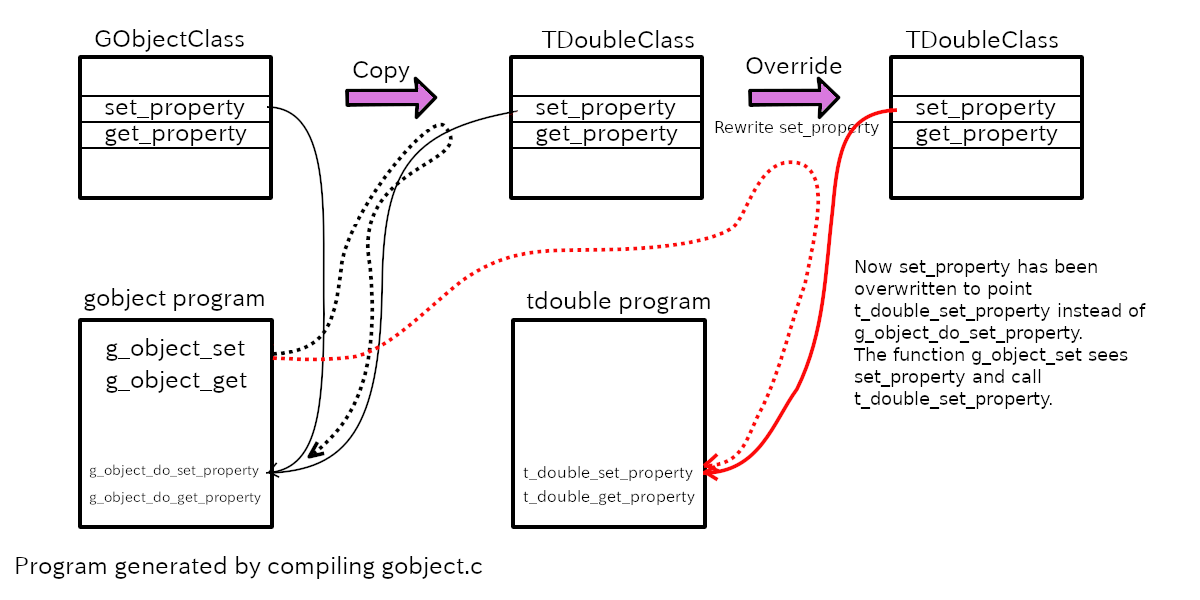
\includegraphics[width=15cm,height=7.5cm]{../image/class_property1.png}
\caption{Overriding \passthrough{\lstinline!set\_property!} class
method}
\end{figure}

The member \passthrough{\lstinline!set\_property!} in GObjectClass class
points \passthrough{\lstinline!g\_object\_do\_set\_property!} in GObject
program, which is made by compiling \passthrough{\lstinline!gobject.c!}.
The GObjectClass part of the TDoubleClass structure (it is the same as
TDoubleClass because TDoubleClass doesn't have its own area) is
initialized by copying from the contents of GObjectClass. Therefore,
\passthrough{\lstinline!set\_property!} in TDoubleClass class points
\passthrough{\lstinline!g\_object\_do\_set\_property!} in GObject
program. But \passthrough{\lstinline!g\_object\_do\_set\_property!}
doesn't store the value to the TDouble instance. The writer of TDouble
object makes \passthrough{\lstinline!t\_double\_set\_property!} function
in \passthrough{\lstinline!tdouble.c!}. And assigns the address of
\passthrough{\lstinline!t\_double\_set\_property!} to
\passthrough{\lstinline!set\_property!} in TDoubleClass class. It is
shown with a red curve in the diagram. As a result,
\passthrough{\lstinline!g\_object\_set!} calls
\passthrough{\lstinline!t\_double\_set\_property!} instead of
\passthrough{\lstinline!g\_object\_do\_set\_property!} (red dotted
curve) and the value will be stored in the TDouble instance. See the
function \passthrough{\lstinline!t\_double\_class\_init!} above. It
changes the member
\passthrough{\lstinline!gobject\_class->set\_property!} to point the
function \passthrough{\lstinline!t\_double\_set\_property!}. The
function \passthrough{\lstinline!g\_object\_set!} sees the TDoubleClass
and call the function pointed by the member
\passthrough{\lstinline!set\_property!}.

The program of \passthrough{\lstinline!t\_double\_set\_property!} and
\passthrough{\lstinline!t\_double\_get\_property!} will shown later.

\subsection{GValue}\label{gvalue}

GValue is generic value. GValue consists of type and value.

The type is any Gtype. The table below shows some GType, but not all.

\begin{longtable}[]{@{}llll@{}}
\toprule\noalign{}
GType & C type & type name & notes \\
\midrule\noalign{}
\endhead
\bottomrule\noalign{}
\endlastfoot
G\_TYPE\_CHAR & char & gchar & \\
G\_TYPE\_BOOLEAN & int & gboolean & \\
G\_TYPE\_INT & int & gint & \\
G\_TYPE\_FLOAT & float & gfloat & \\
G\_TYPE\_DOUBLE & double & gdouble & \\
G\_TYPE\_STRING & & gchararray & null-terminated Cstring \\
G\_TYPE\_PARAM & & GParam & GParamSpec \\
G\_TYPE\_OBJECT & & GObject & \\
G\_TYPE\_VARIANT & & GVariant & \\
\end{longtable}

If the type of a GValue \passthrough{\lstinline!value!} is
\passthrough{\lstinline!G\_TYPE\_DOUBLE!},
\passthrough{\lstinline!value!} can be get with
\passthrough{\lstinline!g\_value\_get\_double!} function.

\begin{lstlisting}[language=C]
GValue value;
value = ... ... ... (a GValue object is assigned. Its type is double.)
double v;
v = g_value_get_double (&value);
\end{lstlisting}

Conversely, you can set GValue \passthrough{\lstinline!value!} with
\passthrough{\lstinline!g\_value\_set\_double!}.

\begin{lstlisting}[language=C]
g_value_set_double (value, 123.45);
\end{lstlisting}

Refer to \href{https://docs.gtk.org/gobject/struct.Value.html}{GObject
API Reference -- GValue} for further information.

\subsection{t\_double\_set\_property and
t\_double\_get\_property}\label{t_double_set_property-and-t_double_get_property}

\passthrough{\lstinline!g\_object\_set!} makes GValue from the value of
the property given as an argument. And calls a function pointed by
\passthrough{\lstinline!set\_property!} in the class. The function is
declared in GObjectClass structure.

\begin{lstlisting}[language=C]
struct  _GObjectClass
{
  ... ... ...
  ... ... ...
  /* overridable methods */
  void       (*set_property)    (GObject        *object,
                                 guint           property_id,
                                 const GValue   *value,
                                 GParamSpec     *pspec);
  void       (*get_property)    (GObject        *object,
                                 guint           property_id,
                                 GValue         *value,
                                 GParamSpec     *pspec);
  ... ... ...
  ... ... ...
};
\end{lstlisting}

\passthrough{\lstinline!t\_double\_set\_property!} just get the value
from GValue \passthrough{\lstinline!value!} and store it to the TDouble
instance.

\begin{lstlisting}[language=C, numbers=left]
static void
t_double_set_property (GObject *object, guint property_id, const GValue *value, GParamSpec *pspec) {
  TDouble *self = T_DOUBLE (object);

  if (property_id == PROP_DOUBLE)
    self->value = g_value_get_double (value);
  else
    G_OBJECT_WARN_INVALID_PROPERTY_ID (object, property_id, pspec);
}
\end{lstlisting}

\begin{itemize}
\tightlist
\item
  3: Casts \passthrough{\lstinline!object!} to TDouble object
  \passthrough{\lstinline!self!}.
\item
  6: Set \passthrough{\lstinline!self->value!}. The assigned value is
  got with \passthrough{\lstinline!g\_value\_get\_double!} function.
\end{itemize}

In the same way, \passthrough{\lstinline!t\_double\_get\_property!}
stores \passthrough{\lstinline!self->value!} to GValue.

\begin{lstlisting}[language=C, numbers=left]
static void
t_double_get_property (GObject *object, guint property_id, GValue *value, GParamSpec *pspec) {
  TDouble *self = T_DOUBLE (object);

  if (property_id == PROP_DOUBLE)
    g_value_set_double (value, self->value);
  else
    G_OBJECT_WARN_INVALID_PROPERTY_ID (object, property_id, pspec);

}
\end{lstlisting}

\subsection{Notify signal}\label{notify-signal}

GObject emits ``notify'' signal when a property is set. When you connect
``notify'' signal to your handler, you can specify a detail which is the
name of the property. The detail is added to the signal name with the
delimiter ``::''.

\begin{lstlisting}[language=C]
g_signal_connect (G_OBJECT (d1), "notify::value", G_CALLBACK (notify_cb), NULL);
\end{lstlisting}

If you don't specify details, the handler is called whenever any
properties are set. So, usually the detail is set.

Notify signal doesn't mean that the value of the property is changed. It
is emitted even if the same value is set. You might want to emit the
notify signal only when the property is actually changed. In that case,
you define the GPramSpec with
\passthrough{\lstinline!G\_PARAM\_EXPLICIT\_NOTIFY!} flag. Then, the
notify signal isn't emitted automatically. Instead you call
\passthrough{\lstinline!g\_object\_notify\_by\_pspec!} function to emit
``notify'' signal explicitly when the value of the property is actually
changed.

It is possible to make setter and getter for the property. But if you
just set the instance member in your setter, notify signal isn't
emitted.

\begin{lstlisting}[language=C]
void
t_double_set_value (TDouble *self, double value) {
  g_return_if_fail (T_IS_DOUBLE (self));

  self->value = value; /* Just set d->value. No "notify" signal is emitted. */
}
\end{lstlisting}

Users must be confused if they want to catch the ``notify'' signal. One
solution is use \passthrough{\lstinline!g\_object\_set!} in your setter.
Then, notify signal will be emitted even if a user uses the setter
function.

\begin{lstlisting}[language=C]
void
t_double_set_value (TDouble *d, double value) {
  g_return_if_fail (T_IS_DOUBLE (d));

  g_object_set (d, "value", value, NULL); /* Use g_object_set. "notify" signal will be emitted. */
}
\end{lstlisting}

The other solution is use
\passthrough{\lstinline!g\_object\_notify\_by\_pspec!} to emit the
signal explicitly. Anyway, if you make a setter for your property, be
careful about notify signal.

\subsection{Define more than one
property}\label{define-more-than-one-property}

If you define more than one property, use an array of property id. It is
good for you to see Gtk source files such as
\passthrough{\lstinline!gtklabel.c!}. GtkLabel has 18 properties.

There's an example in src/tdouble6 directory.

\subsection{Exercise}\label{exercise}

Make TInt object. It is like TDouble but the value type is int. Define
``div-by-zero'' signal and ``value'' property.

Compare your answer to the files in src/tint directory.
